\newpage
\section{Настройка клиентской части}

\subsection{Настройка соединения с БД}

При первом запуске клиентcкой части \tmis~на новой рабочей станции, необходимо выполнить настройку соединения с базой данных. Она может быть сделана без авторизации пользователя в системе. Для этого необходимо в главном меню выбрать пункт \mm{Настройки \str База данных}. Откроется окно настройки соединения (Рисунок \ref{img_cl_db}), где нужно указать параметры соединения с сервером и базой данных. Все поля обязательны для заполнения:
\begin{itemize}
 \item \dm{Тип} – тип СУБД (система управления базами данных, в данном случае используется СУБД MySQL), установленной на сервере, выбирается из списка (в настоящий момент поддерживается только тип сервера MySQL).
 \item \dm{Адрес} – IP-адрес сервера, на котором развернута БД (база данных) \tmis.
 \item \dm{Порт} – номер порта, открытого для соединения с MySQL (при установке MySQL с настройками по умолчанию, используется порт 3306; номер порта может быть изменен с целью обеспечения информационной безопасности).
 \item \dm{База} – название базы данных \tmis, расположенной на сервере; вводится с клавиатуры.
 \item Флажок \dm{Сжимать данные} позволяет уменьшить объем передаваемых данных. Эту опцию рекомендуется использовать при медленном сетевом соединении.
 \item \dm{Имя} – имя пользователя для доступа к БД  \tmis. Разграничение прав пользователей \tmis~производится на уровне приложения. На уровне СУБД все пользователи подключаются, как правило, под одним именем пользователя (например, пользователь <<tmis>>).
 \item \dm{Пароль} – пароль для подключения к БД для указанного выше пользователя.
\end{itemize}

\begin{figure}[ht]\centering
 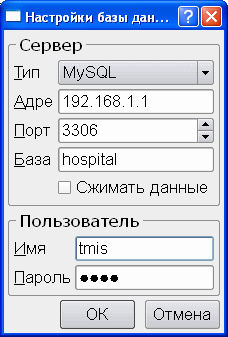
\includegraphics[width = 0.3\textwidth ,keepaspectratio]{cl_db}
 \caption{Настройка соединения с БД}
 \label{img_cl_db}
\end{figure} 

\begin{prim}
 По умолчанию все настройки клиентской части хранятся пользовательском каталоге. Для ОС Windows это папка <<C:$\backslash$Documents and Settings$\backslash$<имя пользователя>$\backslash$ Application Data$\backslash$ftmis-new$\backslash$>>, в файле <<ftmis-new.ini>>. Возможен перенос настроек клиентской части на другую машину простым копированием указанного файла в аналогичную папку на другом компьютере. Для создания нескольких вариантов пользовательских настроек \tmis~на одной рабочей станции, необходимо в операционной системе создать несколько учетных записей пользователей. Для каждой учетной записи возможно сохранение собственных настроек клиентской части.
\end{prim}

\begin{vnim}
 В данном окне и при сохранении настроек соединения проверка доступности подключения не предусмотрена. Для проверки подключения следует в главном меню выбрать пункт \mm{Сессия \str Подключиться к базе данных}.
\end{vnim}

\subsection{Настройки умолчаний}

В разделе \dm{Умолчания} находятся все основные настройки, регулирующие работу пользователя в системе. Настройки данного раздела распространяются только на рабочую станцию (и пользователя), на которой они сохранены. Настройки хранятся в ini-файле профиля пользователя (например, в ОС Windows в папке <<C:$\backslash$Documents and Settings$\backslash$<имя поль\-зо\-ва\-те\-ля>$\backslash$Application Data$\backslash$ftmis-new$\backslash$ftmis-new.ini>>). Для настройки умолчаний нужно в главном меню выбрать пункт \mm{Настройки \str Умолчания}. Окно настройки состоит из нескольких вкладок (Рисунок \ref{img_cl_def}).

\begin{prim}
 В файле <<C:$\backslash$Documents and Settings$\backslash$<имя поль\-зо\-ва\-те\-ля>$\backslash$.ftmis-new$\backslash$error.log>> ведется протоколирование всех ошибок, возникающих на стороне клиента \tmis.
\end{prim}

\begin{figure}[ht]\centering
 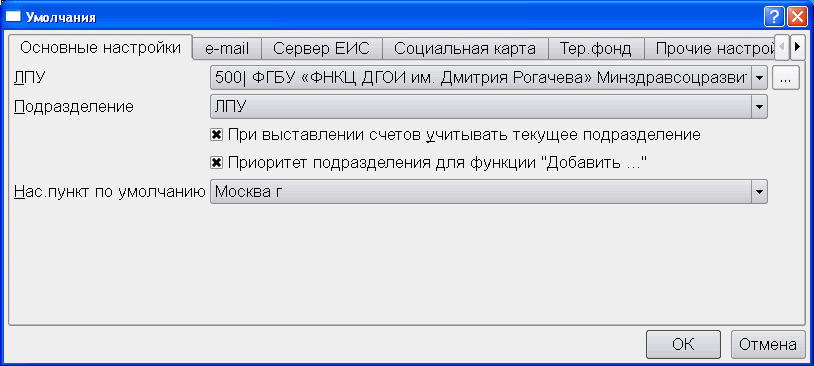
\includegraphics[width = 0.7\textwidth ,keepaspectratio]{cl_def}
 \caption{Настройка умолчаний}
 \label{img_cl_def}
\end{figure} 

На вкладке \dm{Основные настройки} указываются следующие параметры:
\begin{itemize}
 \item \dm{ЛПУ} – наименование базового ЛПУ, выбирается из справочника.
 \item \dm{Подразделение} – подразделение пользователя, выбирается из дерева ЛПУ. При выборе в данном поле значения <<ЛПУ>> для пользователей будет видна информация по всем подразделениям. При выборе определенного подразделения, пользователю будут видны только события и действия, разрешенные в выбранном и нижестоящих подразделениях.
 \item При установке флажка \dm{При выставлении счетов учитывать текущее подразделение} в окне формирования счетов в поле \dm{Подразделение} по умолчанию будет выставлено указанное выше подразделение, т.е. счета будут формироваться только по этому подразделению. При этом формирование счетов по другим подразделениям и ЛПУ в целом остается доступным.
 \item При установке флажка \dm{Приоритет подразделения для функции <<Добавить>>} по умолчанию будут автоматически подставляться действия, доступные для выбранного выше подразделения.
 \item \dm{Нас. пункт по умолчанию} – название населенного пункта следует выбрать из справочника КЛАДР. Данное название будет автоматически подставляться в поле адреса при регистрации новых пациентов, но его можно будет изменить. Данное значение так же будет использоваться для определения иногородних пациентов.
\end{itemize}

\begin{figure}[ht]\centering
 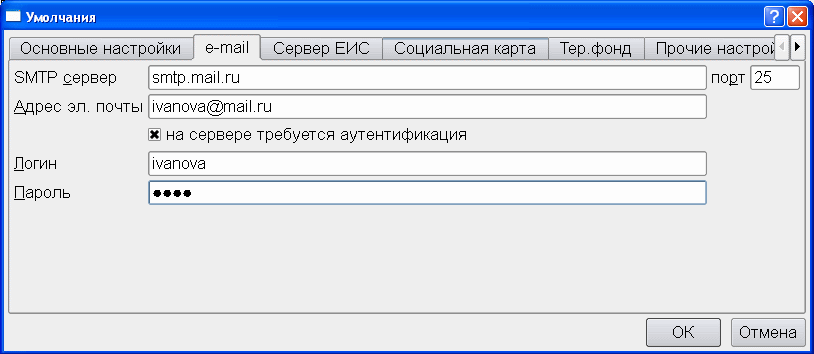
\includegraphics[width = 0.7\textwidth ,keepaspectratio]{cl_def_mail}
 \caption{Настройка почтового клиента}
 \label{img_cl_def_mail}
\end{figure} 

Вкладка \dm{e-mail} (Рисунок \ref{img_cl_def_mail}) содержит настройки встроенного почтового клиента \tmis. Он позволяет отправку отчетов и другой информации непосредственно из \tmis. Для корректной работы почтового клиента необходимо правильно заполнить следующие поля:
\begin{itemize}
 \item \dm{SMTP сервер};
 \item \dm{Порт};
 \item \dm{Адрес эл.почты} полностью;
 \item Флажок \dm{на сервере требуется аутентификация} позволяет ввести логин и пароль для доступа к учетной записи электронной почты;
 \item \dm{Логин} – имя пользователя электронной почты;
 \item \dm{Пароль} – пароль для доступа к электронной почте.
\end{itemize}

\begin{vnim}
 Отправка сообщений по почте возможна только если с текущей рабочей станции доступен SMTP-сервер эл. почты.
\end{vnim}
 
Вкладка \dm{Сервер ЕИС} содержит параметры соединения с сервером ЕИС региона (Рисунок \ref{img_cl_def_eis}). После заполнения всех необходимых полей соединения можно нажать кнопку \btn{Проверить соединение}, что позволит провести тест соединения.

\begin{figure}[ht]\centering
 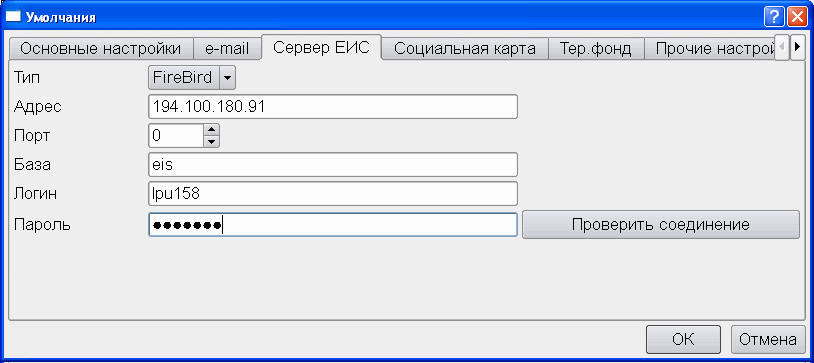
\includegraphics[width = 0.7\textwidth ,keepaspectratio]{cl_def_eis}
 \caption{Настройка соединения с ЕИС}
 \label{img_cl_def_eis}
\end{figure} 

Вкладка \dm{Социальная карта} содержит параметры подключения оборудования и справочников для работы с социальной картой пациента (Рисунок \ref{img_cl_def_sc}). Для того, чтобы поля данной вкладки стали доступны, необходимо установить флажок \dm{Включить поддержку социальной карты} в левом верхнем углу вкладки.

\begin{figure}[ht]\centering
 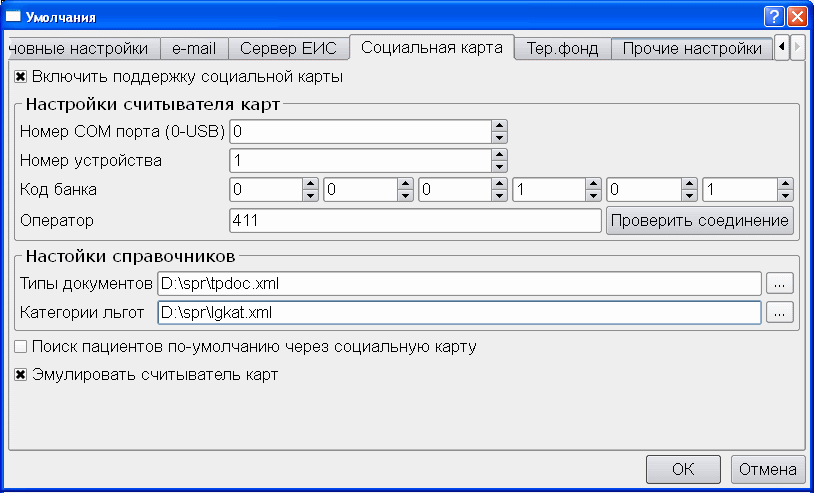
\includegraphics[width = 0.7\textwidth ,keepaspectratio]{cl_def_sc}
 \caption{Настройки работы с социальной картой}
 \label{img_cl_def_sc}
\end{figure} 

На вкладке \dm{Тер.фонд} содержатся настройки соединения с web-сервером ТФОМС региона для проверки действительности полиса пациента в базе застрахованных (Рисунок \ref{img_cl_def_tfoms}). Необходимо указать адрес сервера, а так же логин и пароль для доступа к данным. Для тестирования соединения можно воспользоваться кнопкой \btn{Проверить соединение}.

\begin{figure}[ht]\centering
 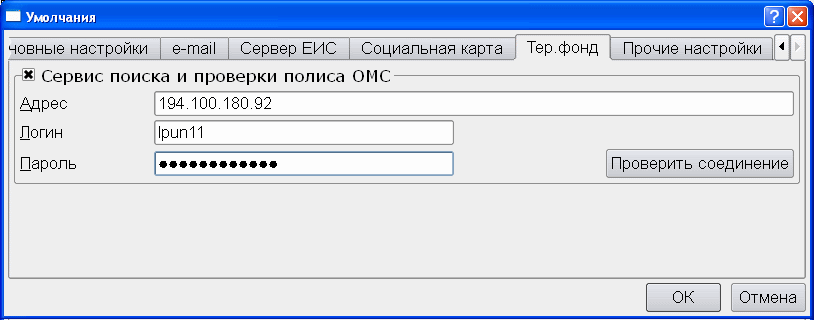
\includegraphics[width = 0.7\textwidth ,keepaspectratio]{cl_def_tfoms}
 \caption{Настройка соединения с сервером ТФОМС}
 \label{img_cl_def_tfoms}
\end{figure} 

Для того чтобы поля данной вкладки стали доступны для редактирования, нужно установить флажок \dm{Сервис поиска и проверки полиса ОМС} в левом верхнем углу вкладки. После установки и сохранения данного флажка в регистрационной карточке пациента, в разделе \dm{Полис ОМС} станет доступной кнопка \btn{Искать}, при нажатии на которую осуществляется поиск полиса в базе данных ТФОМС (Рисунок \ref{img_cl_card_tfoms}).

\begin{figure}[ht]\centering
 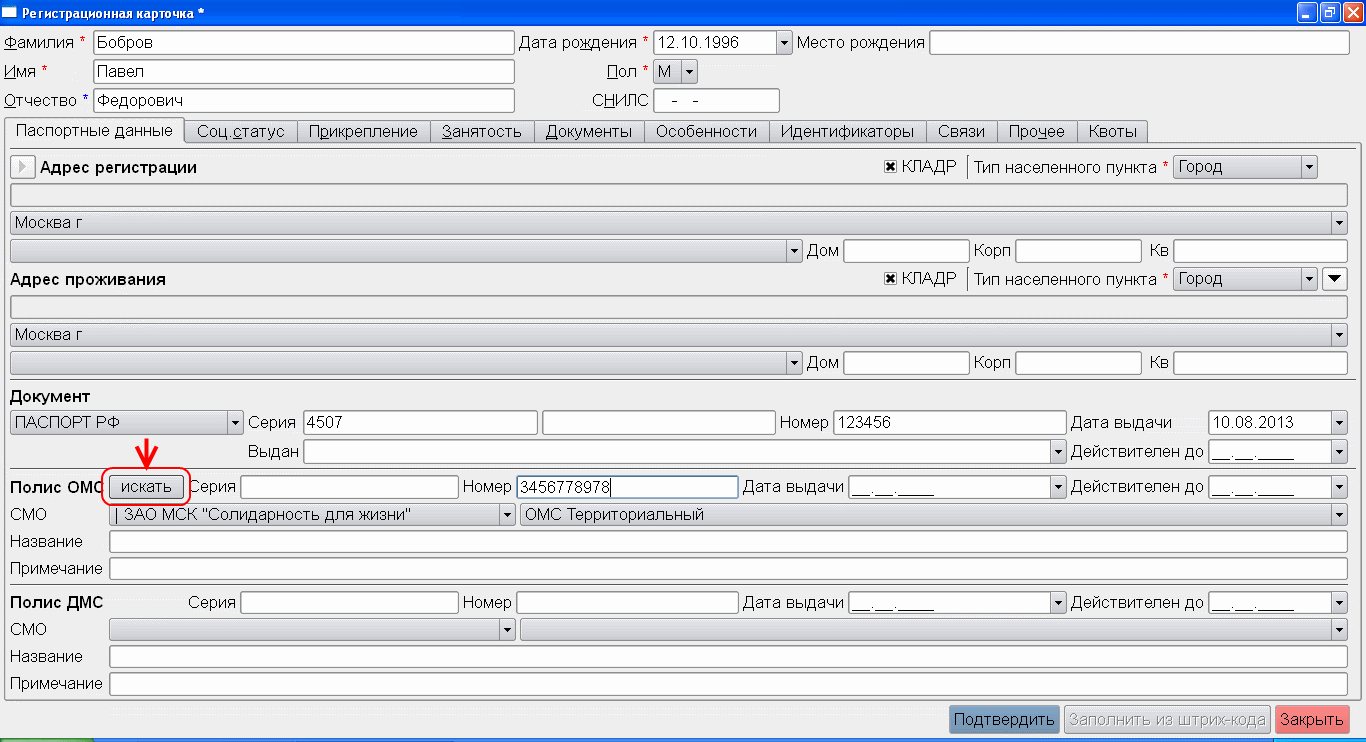
\includegraphics[width = 1\textwidth ,keepaspectratio]{cl_card_tfoms}
 \caption{Кнопка проверки страхового полиса в регистрационной карточке пациента}
 \label{img_cl_card_tfoms}
\end{figure} 

На вкладке \dm{Прочие настройки} содержатся специальные настройки реакции на различные события клиентского приложения (Рисунок \ref{img_cl_def_oth}). Описание опций настройки приведено в таблице \ref{tbl_def1}.

\begin{figure}[ht!]\centering
 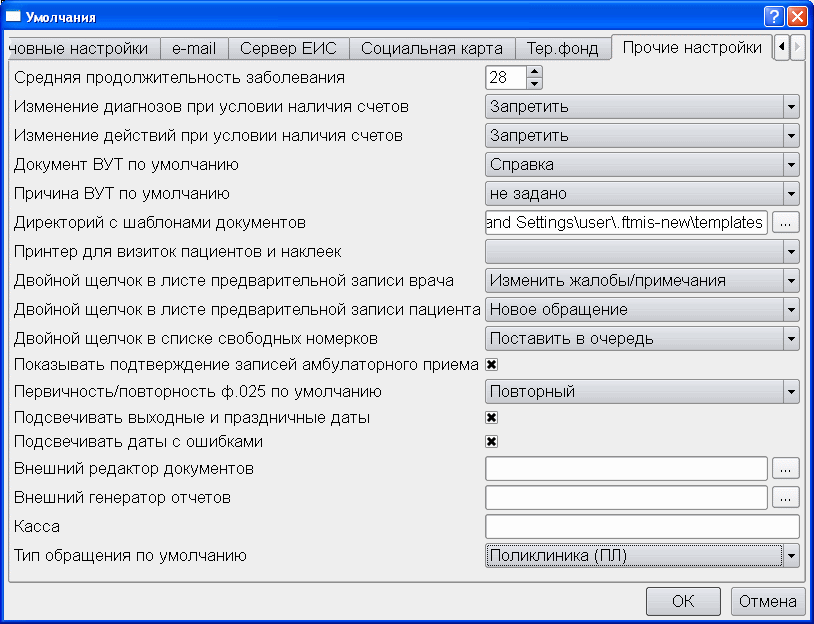
\includegraphics[width = 0.7\textwidth ,keepaspectratio]{cl_def_oth}
 \caption{Вкладка <<Прочие настройки>>}
 \label{img_cl_def_oth}
\end{figure} 

{\small
\begin{longtable}{|p{5cm}|p{11.8cm}|}
\caption{Настройка умолчаний. Вкладка <<Прочие настройки>> \label{tbl_def1}}\\
\hline \rule{0pt}{15pt} \hfil \textbf{Опция} & \hfil \textbf{Описание}\\ \hline
\endfirsthead
\hline \rule{0pt}{15pt} \hfil \textbf{Опция} & \hfil \textbf{Описание}\\ \hline
\endhead
Средняя продолжительность заболевания & Средняя продолжительность заболеваний для отчетов \\ \hline
Количество дней, на редактирование закрытой ИБ & В течении указанного количества рабочих дней после закрытия история болезни будет доступна для редактирования. Рекомендуемое значение -- 2 дня\\ \hline 
Начало учетных суток & Время начала учетных суток в ЛПУ для стационарного монитора \\ \hline
Изменение диагнозов при условии наличия счетов & Разрешает или запрещает изменение диагнозов в обращениях, по которым уже выставлен счет \\ \hline
Изменение действий при условии наличия счетов &	Разрешает или запрещает изменение состава обращения после выставления счета \\ \hline
Документ ВУТ по умолчанию &	Значение, подставляемое по умолчанию при создании документа ВУТ \\ \hline
Причина ВУТ по умолчанию &	Значение, подставляемое по умолчанию при создании документа ВУТ \\ \hline
Директорий с шаблонами документов &	В поле указывается путь к папке с шаблонами печатных форм (в случае их размещения локально). Можно использовать кнопку \btn{\rule{0pt}{5pt}…} для указания пути \\ \hline
Принтер для визиток пациентов и наклеек	& Выбирается из списка принтеров, установленных на данной рабочей станции \\ \hline
Быстрая печать & Использование механизма автоматической отправки на печать на принтер по умолчанию без вывода дополнительных диалогов \\ \hline
Двойной щелчок в лис\-те предварительной записи врача &	Реакция на двойной щелчок мыши на панели \dm{График} по фамилии пациента, записанного на прием (Рисунок \ref{img_cl_def_work}, позиция 1) \\ \hline
Двойной щелчок в лис\-те предварительной записи пациента &	Реакция на двойной щелчок мыши по записи на вкладке \dm{Пациенты} в разделе \dm{Предварительная запись} окна обслуживания пациентов (Рисунок \ref{img_cl_def_work}, позиция 2) \\ \hline
Двойной щелчок в списке свободных номерков	& Реакция на двойной щелчок по свободному номерку на панели \dm{График} или \dm{Номерки} (при условии, что в картотеке пациентов выбран пациент) (Рисунок \ref{img_cl_def_work}, позиция 3) \\ \hline
Показывать подтверждение записей амбулаторного приема	& При установке данного флажка на панели \dm{График} в списке пациентов, записанных на прием, слева от фамилии пациентов появляется дополнительный флажок подтверждения (Рисунок \ref{img_cl_work_acc}) \\ \hline
Первичность/повторность ф.025 по умолчанию	& При создании нового обращения в поле \dm{Первичность} по умол\-ча\-нию указывается выбранное значение \\ \hline
Подсвечивать выходные и праздничные даты	& Во всех полях для указания дат регистрационной карточки пациента, карточки обращения и др. выходные и праздничные дни окрашиваются в красный цвет (Рисунок \ref{img_cl_work_dat}) \\ \hline
Подсвечивать даты с ошиб\-ка\-ми	& Во всех полях для указания дат регистрационной карточки пациента, карточки обращения и др. неправильные (несуществующие) даты окрашиваются в малиновый цвет (Рисунок \ref{img_cl_work_dat}) \\ \hline
Внешний редактор документов	& Путь к исполняемому файлу приложения для редактирования документов (используется для редактирования печатных форм, вызывается из окна предварительного просмотра печатной формы) \\ \hline
Внешний генератор отчетов	& Путь к исполняемому файлу приложения генерации отчетов. Данный редактор вызывается из главного меню \mm{Анализ \str Генератор отчетов} \\ \hline
Касса &	Если рабочая станция расположена в кассе, то в данном поле необходимо ввести с клавиатуры название кассы. Указанное название будет использоваться в качестве названия кассы во всех кассовых операциях \\ \hline
Тип обращения по умолчанию	& При создании нового обращения в поле \dm{Тип обращения} по умолчанию подставляется выбранное значение. Значение выбирается из списка. Состав списка определяется настройкой справочника \dm{Типы обращений} \\ \hline
Порт считывания штрих-кодов & \\ \hline
\end{longtable}
}

\begin{figure}[ht!]\centering
 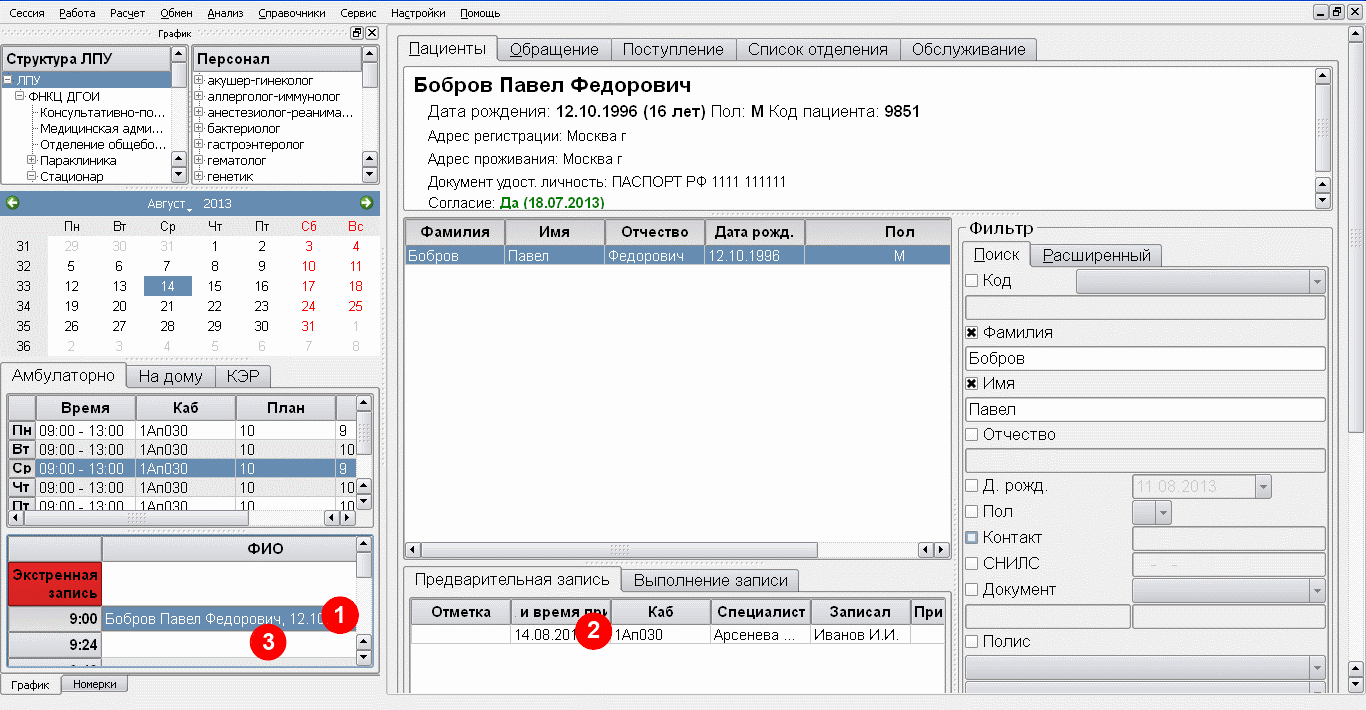
\includegraphics[width = 1\textwidth ,keepaspectratio]{cl_def_work}
 \caption{Позиции, реакция на которые предусмотрена в настройках}
 \label{img_cl_def_work}
\end{figure}

\begin{figure}[ht!]\centering
 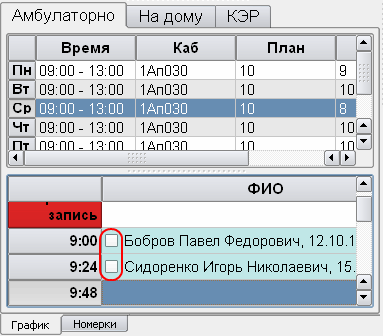
\includegraphics[width = 0.5\textwidth ,keepaspectratio]{cl_work_acc}
 \caption{Подтверждение записей амбулаторного приема}
 \label{img_cl_work_acc}
\end{figure}

\begin{figure}[ht!]\centering
 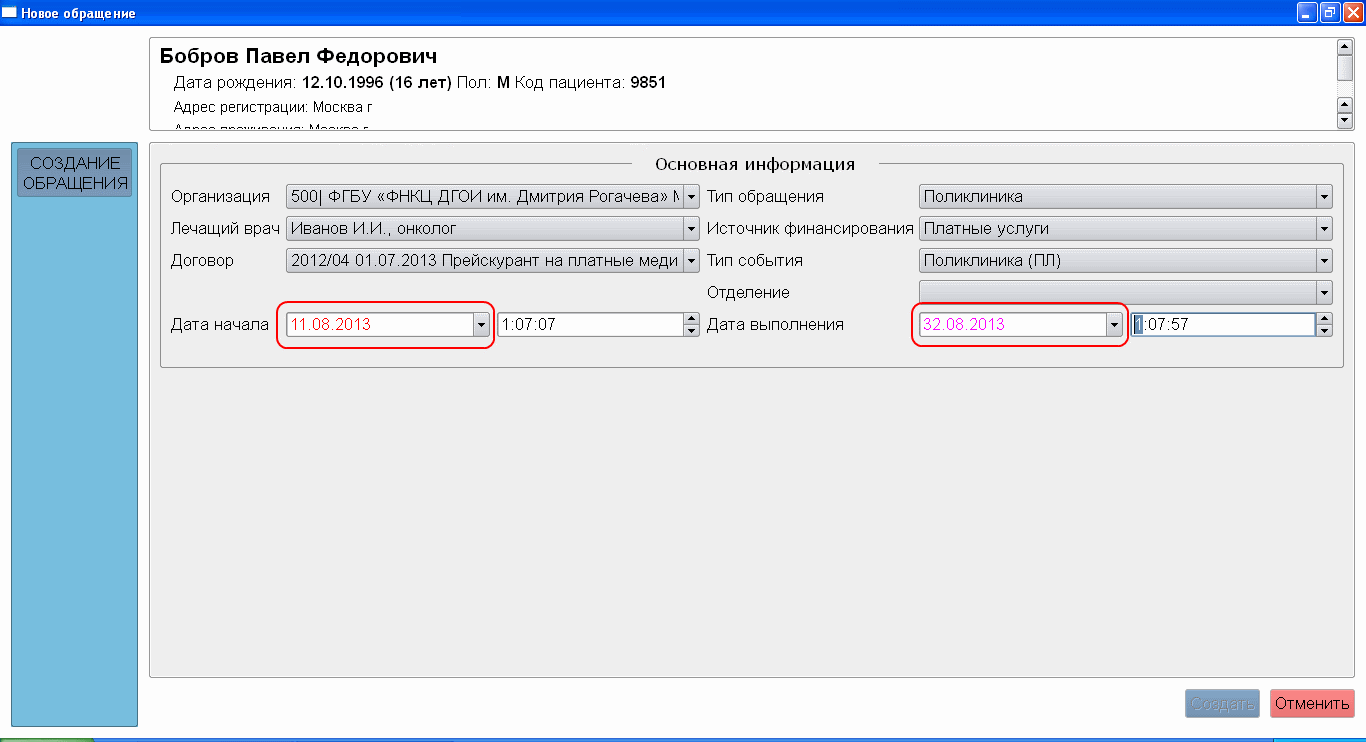
\includegraphics[width = 1\textwidth ,keepaspectratio]{cl_work_dat}
 \caption{Подсвечивание дат}
 \label{img_cl_work_dat}
\end{figure}

\subsection{Настройка внешнего вида}

Настройки внешнего вида приложения так же производится отдельно для каждой рабочей станции. Для открытия окна настройки необходимо в главном меню выбрать пункт \mm{Настройки \str Внешний вид} (Рисунок \ref{img_cl_vid}).

\begin{figure}[ht!]\centering
 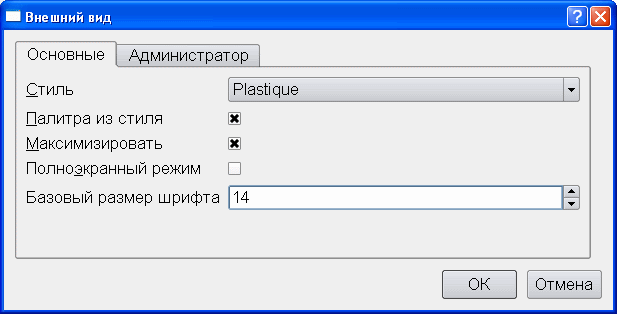
\includegraphics[width = 0.6\textwidth ,keepaspectratio]{cl_vid}
 \caption{Настройка внешнего вида приложения}
 \label{img_cl_vid}
\end{figure}

В открывшемся окне можно указать следующие параметры:
\begin{itemize}
 \item \dm{Стиль} оформления окон приложения выбирается из фиксированного списка стилей.
 \item Флажок \dm{Палитра стиля} позволяет использовать цвета оформления окон, заданные в выбранном стиле.
 \item Флажок \dm{Максимизировать} обеспечивает раскрытие на весь экран окна приложения при запуске.
 \item Флажок \dm{Полноэкранный режим} позволяет запустить приложение во весь экран. Панель задач при этом будет недоступной, а окно приложения невозможно будет свернуть.
 \item \dm{Базовый размер шрифта} – размер шрифта основного текста на экране.
\end{itemize}
 
После внесения изменений, настройки необходимо сохранить, нажав кнопку \btn{OK}.